\documentclass[mathserif, aspectratio=169]{beamer}
\usetheme{odenpecos}
\setbeamertemplate{itemize/enumerate body begin}{\fontsize{8.8}{9}\selectfont}
\setbeamertemplate{itemize/enumerate subbody begin}{\fontsize{7.5}{8}\selectfont}
\setbeamertemplate{itemize/enumerate subsubbody begin}{\fontsize{7.5}{8}\selectfont}

% default search path for figures
\graphicspath{{../2023-11-08-PSAAP-Review/fig}{../fig}}


\newcommand{\zapspace}{\topsep=0pt\partopsep=0pt\itemsep=0pt\parskip=0pt}

\usepackage{multicol}
\usepackage{multirow}
\usepackage{pict2e}
%\usepackage{esdiff}
\usepackage{multimedia}
\usepackage{verbatim}
\usepackage{mhchem}
\usepackage{tikz}
\usetikzlibrary{arrows}
\usepackage[percent]{overpic}
\usepackage[absolute,overlay]{textpos}
\usepackage{tikz} % Required for flow chart
\usepackage[caption=false]{subfig}
\usepackage{tikz} % Required for flow chart
\usepackage[caption=false]{subfig}
\usepackage{pgfplots}

\usepackage{tcolorbox}
\tcbuselibrary{minted,breakable,xparse,skins}
\definecolor{bg}{gray}{0.95}
\DeclareTCBListing{mintedbox}{O{}m!O{}}{%
	breakable=true,
	listing engine=minted,
	listing only,
	minted language=#2,
	minted style=default,
	minted options={%
		linenos,
		gobble=0,
		breaklines=true,
		breakafter=,
		fontsize=\small,
		numbersep=8pt,
		#1},
	boxsep=0pt,
	left skip=0pt,
	right skip=0pt,
	left=25pt,
	right=0pt,
	top=3pt,
	bottom=3pt,
	arc=5pt,
	leftrule=0pt,
	rightrule=0pt,
	bottomrule=2pt,
	toprule=2pt,
	colback=bg,
	colframe=orange!70,
	enhanced,
	overlay={%
		\begin{tcbclipinterior}
			\fill[orange!20!white] (frame.south west) rectangle ([xshift=20pt]frame.north west);
	\end{tcbclipinterior}},
	#3,
}

\newcommand{\overbar}[1]{\mkern 1.5mu\overline{\mkern-1.5mu#1\mkern-1.5mu}\mkern 1.5mu}
\newcommand{\pp}[2]{\frac{\partial #1}{\partial #2}}
\newcommand{\dd}[2]{\frac{d #1}{d #2}}
\newcommand{\DD}[2]{\frac{D #1}{D #2}}
\newcommand{\mm}{\mathbf{minmod}}
\def\etal{{\it et al~}}
\newcommand{\be}{\begin{eqnarray}}
	\newcommand{\ee}{\end{eqnarray}}
\newcommand{\mbb}[1]{\mathbb{#1}} % math blackboard bold
\newcommand{\mcal}[1]{\mathcal{#1}} % math blackboard bold
\newcommand{\mbf}[1]{\mathbf{#1}} % math bold face (for vectors)
\newcommand{\sbf}[1]{\boldsymbol{#1}} % bold face for symbols
\newcommand{\jump}[1]{\llbracket #1 \rrbracket} % jump operator
\newcommand{\avg}[1]{\langle #1 \rangle} % average operator
\newcommand{\rarrow}{\rightarrow}
\newcommand{\Rarrow}{\Rightarrow}
\newcommand{\LRarrow}{\Leftrightarrow}
\newcommand{\vvvert}{|\kern-1pt|\kern-1pt|}
\newcommand{\enorm}[1]{\vvvert #1 \vvvert}
\newcommand{\nutil}{\tilde{\nu}}
\newcommand{\Var}{\mathrm{Var}}
\newcommand{\Cov}{\mathrm{Cov}}


\definecolor{MyDarkGreen}{rgb}{0,0.45,0.08}
\newcommand{\myred}[1]{{\color{red} #1}}
\newcommand{\myblue}[1]{{\color{blue} #1}}
\newcommand{\mygreen}[1]{{\color{MyDarkGreen} #1}}

\newcommand{\sa}{\nu_{\mathrm{sa}}}
\newcommand{\tep}{\tilde{\epsilon}}
\newcommand{\Ssd}{\mathcal{S}} % source term due to slow derivative
\newcommand{\ud}{\,\mathrm{d}}

\newcommand{\Mach}[1]{\ensuremath{\mbox{Ma}_{#1}}}
\newcommand{\Reynolds}{\ensuremath{\mathit{Re}}}
\newcommand{\DensityRat}{\ensuremath{\mathit{DR}}}
\newcommand{\BlowRat}{\ensuremath{\mbox{BR}}}
\newcommand{\VelRat}{\ensuremath{\mathit{VR}}}
\newcommand{\Tau}{\ensuremath{\mathrm{T}}}

\newcommand{\wall}     {\ensuremath{\mathrm{w}}}   % wall subindex
\newcommand{\awall}    {\ensuremath{\mathrm{aw}}}  % adiabatic wall subindex

\newcommand{\commentout}[1]{}

\newcommand{\vect}[1]{\boldsymbol{#1}}
\usepackage{mleftright}
\newcommand{\of}[1]{\mleft( #1 \mright)}
\newcommand{\vth}{v_{\textrm{th}}}
\newcommand{\reals}{\mathbb{R}}
\newcommand{\myint}{\int\limits}
\newcommand{\ddt}[1]{\partial_t #1}
\newcommand{\RR}{\mathbb{R}}
\newcommand{\vr}{v}
\newcommand{\diff}[1]{\, d#1}
\newcommand{\norm}[1]{\left\lVert#1\right\rVert}
%\newcommand{\vtheta}{\theta_{\vect{v}}}
%\newcommand{\vphi}{\varphi_{\vect{v}}}
%\newcommand{\vr}{v_{r}}
\newcommand{\vtheta}{{v_{\theta}}}
\newcommand{\vphi}{v_{\varphi}}
\newcommand{\vomega}{v_{\omega}}
\newcommand{\vrunit}{\hat{\vect{v}}_{r}}
\newcommand{\vthetaunit}{\hat{\vect{v}}_{\theta}}
\newcommand{\vphiunit}{\hat{\vect{v}}_{\varphi}}
\DeclareMathOperator{\variance}{Var}

\usepackage{mathtools}
\DeclarePairedDelimiter\ceil{\lceil}{\rceil}
\DeclarePairedDelimiter\floor{\lfloor}{\rfloor}

\begin{document}
% disable nav
\setbeamertemplate{navigation symbols}{}

% ---------------------------------------------------------------
% Oden/Pecos title page

\hoffset=.16in

\begin{frame}[plain,t]{}
\makeatletter
%\vspace*{0.85cm}
%\vspace*{0.65cm}
\includegraphics[height=0.9in,trim=50 40 40 0, clip]{PMSc_159_university_formal_horizontal.pdf} \newline
%\vspace*{0.3cm}
\begin{columns}[T,onlytextwidth]
\column{.8\textwidth}
{\bf \color{burntorange} \fontfamily{bch}\selectfont 
% -- Set talk title here
Solving the Boltzmann Equation for Electron Kinetics Using Galerkin Approach %using Galerkin approach
% --
}
\end{columns}
\vspace*{.15cm}
\rule{.8\textwidth}{0.6pt} \newline

\vspace*{0.05cm}
\setstretch{0.65}
{\fontfamily{phv}\selectfont
  { \scriptsize
    % -- define presenter, authors here
    \textbf{Milinda Fernando}, George Biros, Todd Oliver, Laxminarayan Raja\\ Philip Varghese, Robert Moser \\%, Todd Oliver, Laxminarayan Raja, Philip Varghese, Robert Moser, George Biros  \\
    % --
  }
  {\color{burntorange} \tiny
    % -- define role, meeting event, location, etc
    PSAAP III Annual Review $\cdot$ November 08-09, 2023
    %PSAAP TST Meeting $\cdot$ April 24-25, 2023
    % --
  }
}

\vspace*{1cm}
%\includegraphics[height=0.3in]{figures/pecos_orange1.png}
\begin{columns}
\begin{column}{0.8\linewidth}
\includegraphics[height=0.5in]{oden_pecos_2020_wordmark.png}\\
{\scriptsize \url{https://pecos.oden.utexas.edu}}
\end{column}

\begin{column}{0.2\linewidth}
\includegraphics[height=0.6in]{psaap3-logo.png}
\end{column}
\end{columns}

\end{frame}
\hoffset=0in
% -- end title slide ---------------------------------------------

%\begin{frame}
%	\frametitle{Outline}
%	\begin{itemize}
%		\item Spatially homogeneous Boltzmann equation, $\partial_t f - \frac{\vect{E} q}{m} \cdot \nabla_{\vect{v }}f = C(f)$
%		\item Representation of $f$ (i.e., isotropic + anisotropic correction terms), use spherical harmonics for angular directions + experimentation of basis functions in radial direction. 
%		\begin{itemize}
%			\item Global approximations with Maxwell and Laguerre polynomials.
%			\item Local approximations with linear and higher order B-splines
%		\end{itemize}
%		\item Collision operator (5d integral form)
%		\item Simplifications for the collision operator with analytical integration of angular directions (1d integral form). 
%		\item Equations for the steady-state solution (spatially homogeneous case) 
%		\item Two-term formulation vs. EEDF formulation with diffusion term. 
%		\item Verification with Bolsig+ code.  (Both approaches, importance of the diffusion term), PS 2.4
%		\item Formulation for 1D-space+3D-velocity space Boltzmann equations with some preliminary results for 1d glow discharge problem. 
%		\item Discuss on single GPU implementation with CuPy, Challenges in 1D+3V formulation (i.e., boundary conditions) and Future work, ES 2.6
%	\end{itemize}
%\end{frame}

%\begin{frame}[fragile]
%	\frametitle{Where do we fit ? }
%	% \begin{tikzpicture}
%	% 	\node[anchor=south west,inner sep=0] at (0,0) {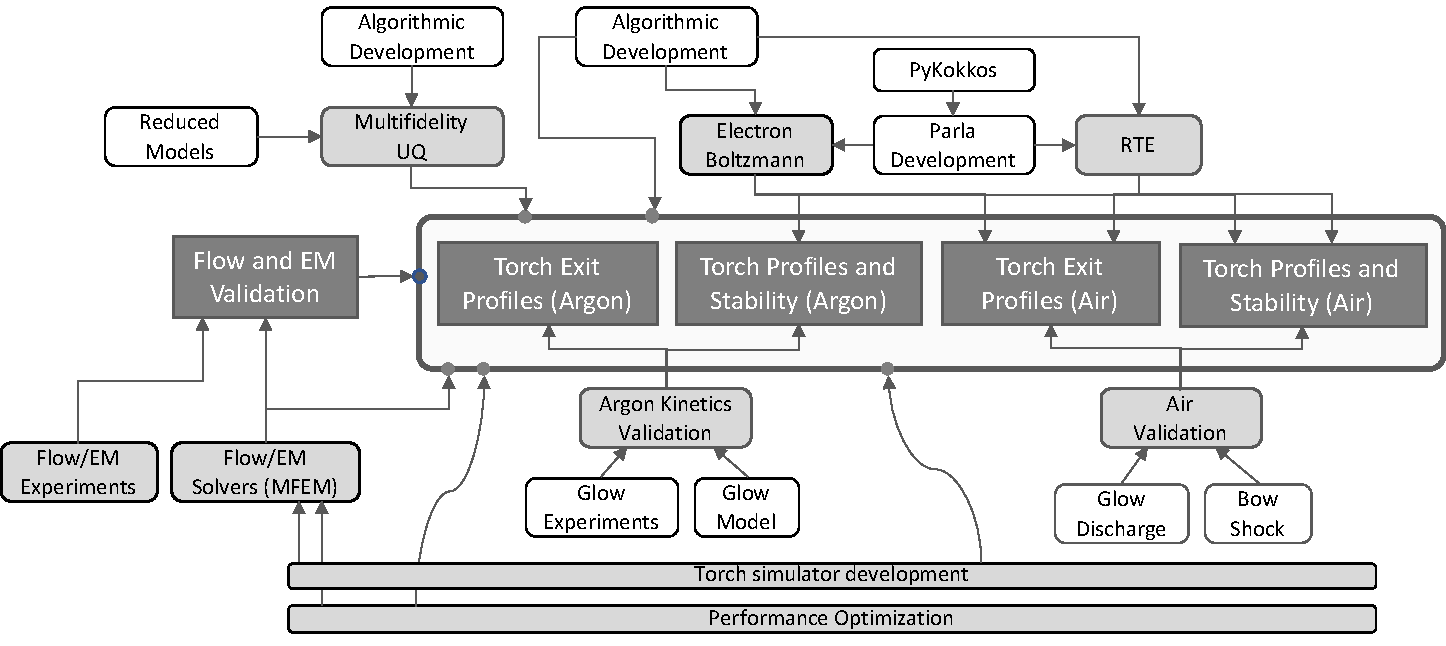
\includegraphics[width=0.8\textwidth]{pecos_roadmap_tst_1.5.pdf}};
%	% 	\draw[orange, fill = yellow!30, fill opacity = 0.4 ,ultra thick,rounded corners] (4.15,3.6) rectangle +(4.2,1.6);
%	% \end{tikzpicture}
%	\begin{center}
%		\includegraphics[width=0.9\textwidth]{where_we_fit.png}
%	\end{center}
%\end{frame}

\begin{frame}
	\frametitle{Outline}
	\begin{center}
		\begin{itemize}
			\item 0D-space BTE (spatially homogeneous case)
			\item Formulation \& Discretization
			\item Collision operators
			\begin{itemize}
				\item $C_{en}$ : electron-heavy 
				\item $C_{ee}$ : electron-electron Coulomb
			\end{itemize}
			\item Steady-state solutions
			\item Verification
			\item 0D-Batched BTE solver
			\item 1D-space BTE
		\end{itemize}
	\end{center}
\end{frame}

%\begin{frame}
%	\frametitle{Outline}
%	\begin{columns}
%		\begin{column}{0.4\textwidth}
%				\begin{itemize}
%				\item Spatially homogeneous BTE
%				\item Formulation \& discretization
%				\item Collision operators
%				\begin{itemize}
%					\item electron-heavy collisions
%					\item electron-electron collisions
%				\end{itemize}
%				\item Steady-state solutions
%				\item Verification with Bolsig
%			\end{itemize}
%		\end{column}
%		\begin{column}{0.6\textwidth}
%			\begin{itemize}
%				\item Year 1 : Discretization and formulation 
%				\begin{itemize}
%					\item B-Splines + Spherical harmonics
%				\end{itemize}	
%				\item Year 2 : Verification with Bolsig
%				\item Year 3 : Torch + Boltzmann coupling
%					\begin{itemize}
%						%\item Issues with the boundary condition
%						\item electron-electron collisions + anisotropic EEDF
%						\item Explore 1D-space Boltzmann
%					\end{itemize}
%			\end{itemize}
%			\vspace{0.25in}
%			\textbf{Developments from last review}
%				\begin{itemize}
%					\item Beyond 2-term approximation
%					\item Verification with Bolsig+, PIC-DSMC code with new features
%					\item Efficient steady-state solver
%					\item Batched 0D-Boltzmann solver (steady-state and transient)
%					\item Integration with TPS + Parla + MPI
%					%\item Implementation of 1d2v glow-discharge with Boltzmann
%					%\item 0D-Boltzmann paper
%				\end{itemize}
%		\end{column}
%	\end{columns}
%\end{frame}



\begin{frame}
	\frametitle{Boltzmann transport equation}
	\begin{align}
		\partial_t f  + \underbrace{\vect{v} \cdot \nabla_{\vect{x}} f}_{\textcolor{orange}{\text{spatial advection}}} -\underbrace{\frac{\vect{E} q}{m} \cdot \nabla_{\vect{v }}f}_{\textcolor{orange}{\text{Acceleration due to $\vect{E}$ field}}} = \underbrace{C_{en}f + C_{ee}(f)}_{\textcolor{orange}{\text{underlying collisions}}}
	\end{align}
	\begin{itemize}
		\item $\nabla_{\vect{x}} f =0$ (spatially homogeneous assumption), $f(t, \vect{v})$
		\item $C_{en}$ : electron-heavy collisions: elastic, excitation, ionization, $e + X \rightarrow k e + Y$
		\begin{itemize}
			\item Use LXCAT cross-section data 
			\item Linear in $f$
		\end{itemize} 
		\item $C_{ee}$ : electron-electron Coulomb collisions 
		\begin{itemize}
			\item Modeled using Fokker-Plank equation with analytical cross-section
			\item Nonlinear in $f$
		\end{itemize}
%		\item $C_{re}$ : 3-body recombination 
%		\begin{itemize}
%			\item Implemented in PIC-DSMC solver
%			\item Under development for deterministic grid BTE solver
%		\end{itemize}
		%\item $C_{ei}$: electron-ion Columbic can be modeled similarly if needed
%		\item Derived the steady state equation
%		\begin{align}
%			\textcolor{black!70}{\partial_t \hat{f} = -(u^T C \hat{f}) \hat{f} + (C+E)\hat{f} \text{ where } \hat{f}(\vect{v},t) = \frac{f(v,t)}{\myint_{R^3} f(\vect{v},t) \diff{\vect{v}}}}\\
%			\textcolor{black!70}{\partial_t (\hat{f}) = 0 \ \ \  \Rightarrow} \ \ \  -(u^T C \hat{f}) \hat{f} + (C+E)\hat{f} =0  \text{ with } u^T \hat{f}-1=0
%		\end{align}
	\end{itemize}
\end{frame}

\begin{frame}
	\frametitle{Challenges}
	\begin{columns}
		\begin{column}{0.3\textwidth}
			\begin{itemize}
				\item Non-smooth cross-sections $\Rightarrow$ non-smooth $f$ solutions
				\item Strong advection may cause stabilization issues
				\item To compute QoIs $\rightarrow$ need accurate tails of $f$ 
			\end{itemize}
		\end{column}
		\begin{column}{0.7\textwidth}
			\vspace*{-0.8in}
			\begin{center}
				\includegraphics[width=\columnwidth]{g0_g2_cs.png}
			\end{center}
		\end{column}
	\end{columns}
\end{frame}

\begin{frame}
	\frametitle{$\vect{v}$-space discretization (spherical coordinates)}
	\small
	\begin{itemize}
		\item Representation of $f\of{\vect{v},t} = \sum_{klm} f_{klm} \underbrace{\phi_k\of{v}}_{\text{B-Spline basis}} \underbrace{Y_{lm}\of{v_\theta, v_\phi}}_{\tiny\text{sph. harm.}}$ 
		\item Weak formulation
			$
			\displaystyle
			\quad
			\partial_t f - \frac{\vect{E} q}{m} \cdot \nabla_{\vect{v}}f = C(f)
			\quad $ \\
			$
			\displaystyle
			\quad
			\Rightarrow \quad
			\partial_t \myint_{R^3} f \phi\of{\vect{v}} \ud \vect{v} = 
			\myint_{R^3} \of{C_{en}f + C_{ee}(f)} \phi\of{\vect{v}} \ud \vect{v} + \myint_{R^3} \of{\frac{\vect{E} q}{m} \cdot \nabla_{\vect{v}} f} \phi(\vect{v}) \ud \vect{v}\text{ , } 
			\forall \phi(\vect{v})$
		\item Weak form of the collision operator (5d integral) \\
			$
			\displaystyle
			\quad 
			\myint_{R^3} C_{en} \phi\of{\vect{v}_e} \diff{\vect{v}_e} 
			=
			N \myint_{R^3} \myint_{S^2} 
			v\sigma(v,\vect{\omega})
			f_e\of{\vect{v}_e}
			\left(
			\psi\of{\vect{v}_e^\text{post}\of{\vect{v}_e, \vect{\omega}}} 
			- \psi\of{\vect{v}_e} 
			\right)
			\diff{\vect{v}_e} \diff{\vect{\omega}}
			$
		\item Isotropic scattering, azimuthal symmetry, and using spherical harmonics addition theorem\\
		$
		\displaystyle
		\quad 
		C_{en}^{ql} 
		=
		N \myint_{0}^{\infty} 
		v^3\sigma(v)\delta_{ql}
		f_e^{l}\of{v}
		\left(
		\delta_{q0}\psi\of{v_e^\text{post}\of{v}} - \psi\of{v} 
		\right)
		\diff{v} 
		$ 
	\end{itemize}
\end{frame}

\begin{frame}
	\frametitle{Electron-electron  Coulomb collisions}
	\begin{itemize}
		\item We use Rosenbluth's (1957) Fokker-Plank derivation for electron-electron collisions. Let $H=\partial^2_{ab}$
		\begin{align}
			C_{ee}(f) &= \Gamma_a(-\nabla \cdot (f \nabla h ) + \frac{1}{2} H : \of{f H g}) \text{ where } \Delta h  = -8\pi f \text{ and } \Delta^2 g =-8\pi f	
		\end{align}
		\item Assuming azimuthal symmetry, we can compute Rosenbluth potentials, 
		\begin{align}
			& h_a\of{\vect{v}} = \sum_{l} A^{b}_l\of{v} Y_{l0}\of{\vtheta, \vphi}  \text{ and } g\of{\vect{v}} = \sum_{l} B^{b}_l\of{v} Y_{l0}\of{\vtheta, \vphi}\text{ where } \\
			\tiny
			& A^{b}_l\of{v} = \frac{8\pi}{(2l+1)}\of{\int_{0}^{v} dv^\prime \frac{{v^\prime}^{l+2}}{v^{l+1}} f^{b}_l\of{v^\prime} +  \int_{v}^{\infty} dv^\prime \frac{{v}^{l}}{{v^\prime}^{l-1}} f^{b}_l\of{v^\prime}}\\
			\tiny
			B^{b}_{l}\of{v} & = -\frac{4\pi}{(4l^2-1)} \of
			{
				\int_{0}^{v} \diff{v^\prime} f^{b}_l\of{v^\prime} \frac{{v^\prime}^{l+2}}{v^{l-1}} \of{1 - \of{\frac{l-1/2}{l+3/2}}\of{\frac{{v^\prime}^2 }{v^2}}} } + \hdots% \nonumber\\
			% &-\frac{4\pi U_{l0}}{(4l^2-1)} \of{
			% 	\int_{v}^{\infty} \diff{v^\prime} f^{b}_l\of{v^\prime} \frac{{v}^{l}}{{v^\prime}^{l-3}} \of{1 - \of{\frac{l-1/2}{l+3/2}}\of{\frac{{v}^2 }{{v^\prime}^2}}}
			% }
		\end{align}
		\item \textbf{Take away} : \textcolor{orange}{$h$, and $g$ are moments of $f$, can be pre-computed}
	\end{itemize}
\end{frame}

\begin{frame}
	\frametitle{Pre-computed operators}
	\begin{itemize}
		\item Electron-heavy and $\vect{v}$-space advection $\implies$ matrices (after Galerkin discretization)
		\item Weak form of the Coulomb collisions
		\begin{itemize}
			\item 
			\begin{align}
				\int_{R^3} C_{ee}(f) \psi(\vect{v})\diff{\vect{v}} = \Gamma_a \of{\int_{R^3} \nabla \psi\of{\vect{v}} \cdot (f \nabla h ) 	\diff{\vect{v}}  + \frac{1}{2} \int_{R^3} H\psi\of{\vect{v}} : \of{f H g} \diff{\vect{v}}} 
			\end{align}
			\item For given test function $\psi_{pq}$, we can pre-compute 6-th order tensor ${C_{ee}}_{rs,kl}^{pq}$
			\begin{align}
				[C_{ee}]_{rs,kl}^{pq} = \int_{R^3} C_{ee}(\phi_{rs}, \phi_{kl}) \psi_{pq} \diff{\vect{v}} 
			\end{align}
			\item SymPy based symbolic framework %for weak form derivation in spherical coordinates
		\end{itemize}
		\item To solve $\implies$ apply matrix and tensor operations on vectors $\implies$ easily mapped CPU and GPUs through exciting math libraries
%		\begin{itemize}
%			\item Ability to derive equation for arbitrary number of polar modes
%			\item Integrate the angular coordinates analytically %, identification of the non-zero modes (i.e., sparse tensor) 
%			\item \textbf{Sparsification} tensor
%			%\item Radial integration performed exactly using Gauss quadrature on B-Splines
%		\end{itemize}
	\end{itemize}
\end{frame}

\begin{frame}
	\frametitle{Transient and steady-state solutions}
	\begin{itemize}
		\item Steady-state solution for a given $E/N$ field and ionization degree $n_e/N$ 
		\begin{align}
			\partial_t {\hat{f}} &=(C_{en}+E)\hat{f} + n_e C_{ee}\of{\hat{f}} - \mu(\hat{f}) \hat{f} \text{ where } \mu(\hat{f}) = \frac{\partial_t n_e}{n_e} = u^T C_{en}(\hat{f})\\
			&\text{ with constraint } u^T \hat{f} = 1 \nonumber 
		\end{align}
		\item Steady-state: Newton's method with line search
		\item Transient: Implicit time integration
%		\item For steady-state solution we solve $\partial_t {\hat{f}} = 0$, with $R(\hat{f}) = (C_{en}+E)\hat{f} + n_e C_{ee}\of{\hat{f}, \hat{f}} - \mu(\hat{f})$, we can write the Jacobian $\frac{d R}{d\hat{f}} = J(\hat{f}) = C_{en} + E + n_e \of{C_{ee}\of{\cdot,\hat{f}} + C_{ee}\of{\hat{f},\cdot}} -\mu(\hat{f})I$
		%\item $\hat{f}^{n+1} = \hat{f}^{n} - \alpha [J(\hat{f}^n)]^{-1}R(\hat{f}^n)$, where $\alpha \in(0,1]$ determined by line-search algorithm 
	\end{itemize}
	\textit{Both are novel numerical schemes for BTE}
\end{frame}

\begin{frame}
	\frametitle{Electron-electron Coulomb collisions}
	$E/N$ = 1Td with elastic + ionization; varying ionization degree $n_e/N$
	\vspace*{-0.08in}
	\begin{center}
		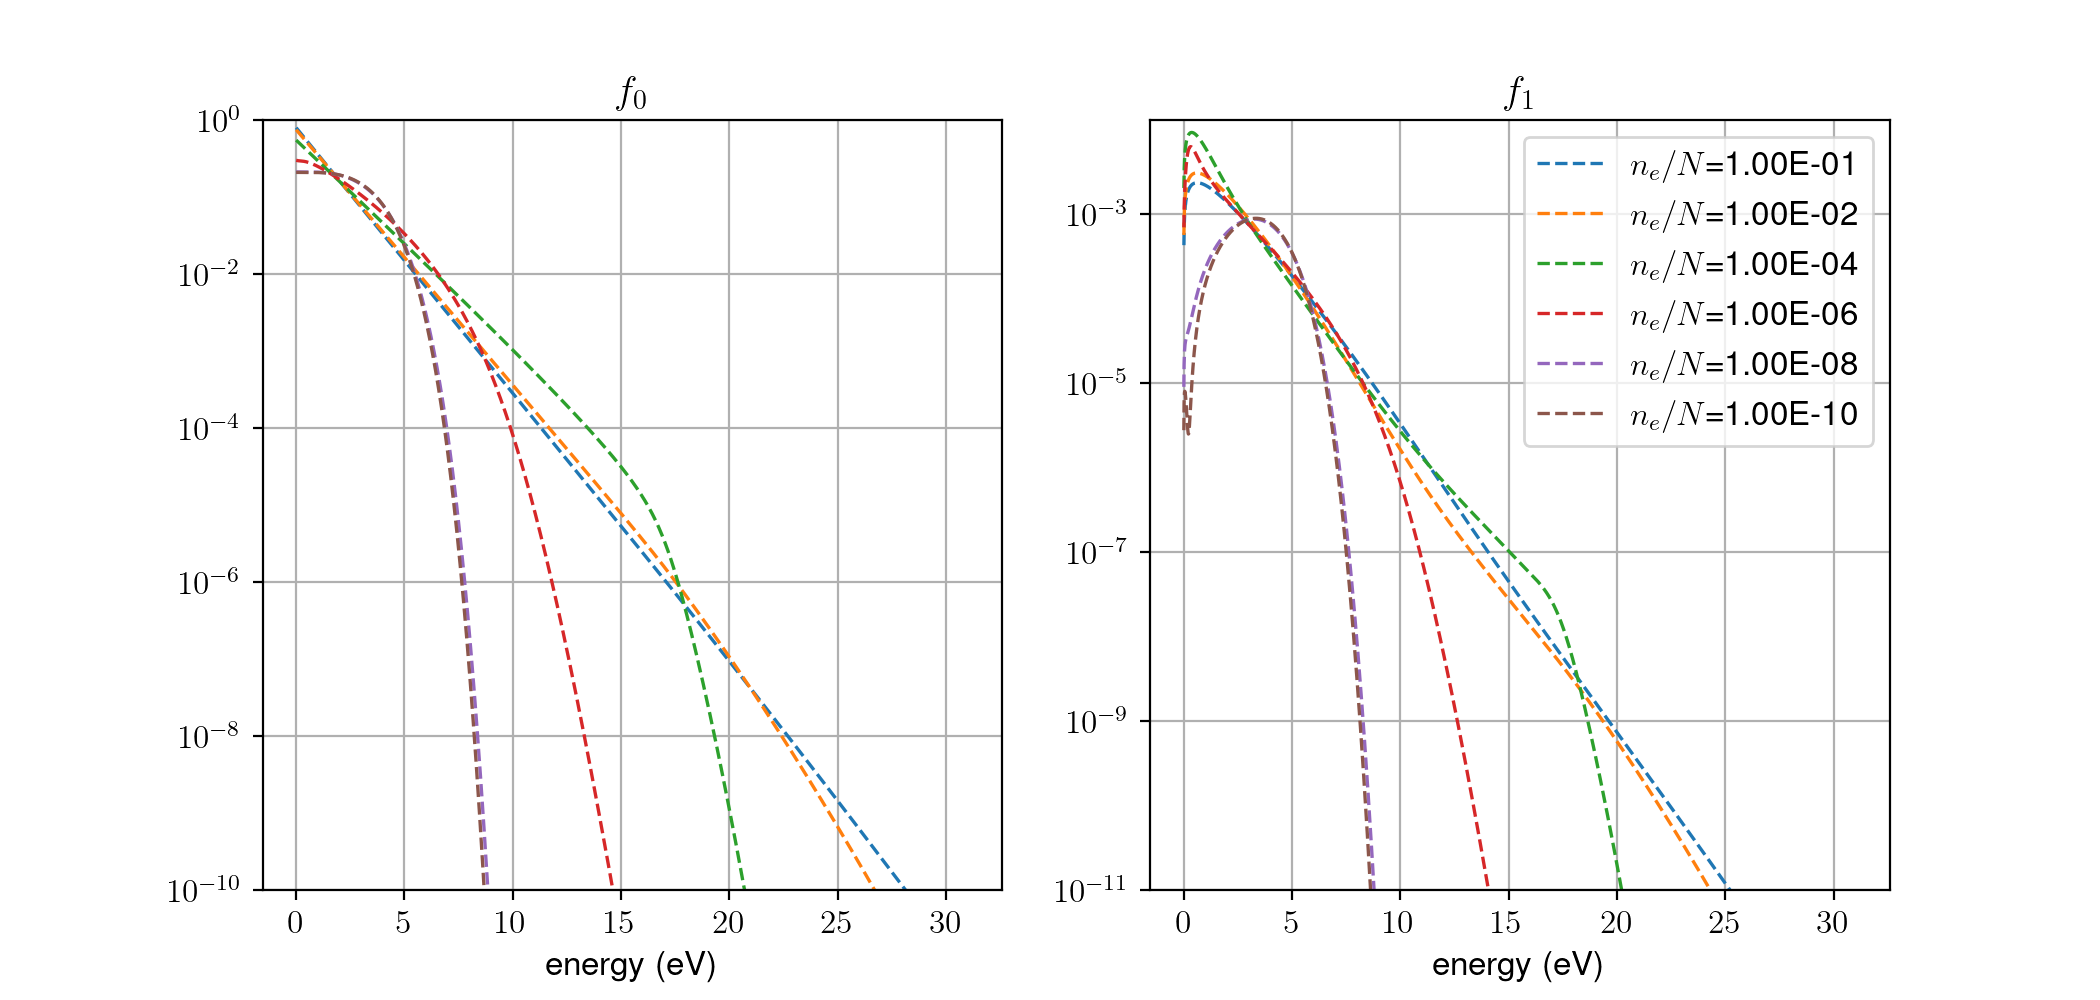
\includegraphics[width=0.9\textwidth]{1Td_cc.png}
	\end{center}
\end{frame}

\begin{frame}
	\frametitle{Verification}
	\begin{itemize}
		\item Bolsig+: fixed two term approximation $f(\vect{v},t) = f_0(v, t) + f_1(v,t)\cos v_\theta$, %assumes higher order correction terms negligible
		\item Compare with Bolsig+\footnote[frame]{Hagelaar, G.J.M. and Pitchford, L.C., 2005. Solving the Boltzmann equation to obtain electron transport coefficients and rate coefficients for fluid models. Plasma sources science and technology, 14(4), p.722.} and PIC-DSMC (for multi-term approximation)\footnote[frame]{Almgren-Bell, J., Al Awar, N., Geethakrishnan, D.S., Gligoric, M. and Biros, G., 2022, November. A Multi-GPU Python Solver for Low-Temperature Non-Equilibrium Plasmas. In 2022 IEEE 34th International Symposium on Computer Architecture and High Performance Computing (SBAC-PAD) (pp. 140-149). IEEE.} code for verification step 
		\item Finite differences with uniform grid in energy
		\item Supports steady-state and time-harmonic solutions
	\end{itemize}
\end{frame}

%\begin{frame}[fragile]
%	\frametitle{Verification with Bolsig+}	
%	\begin{center}
%		\only<+>{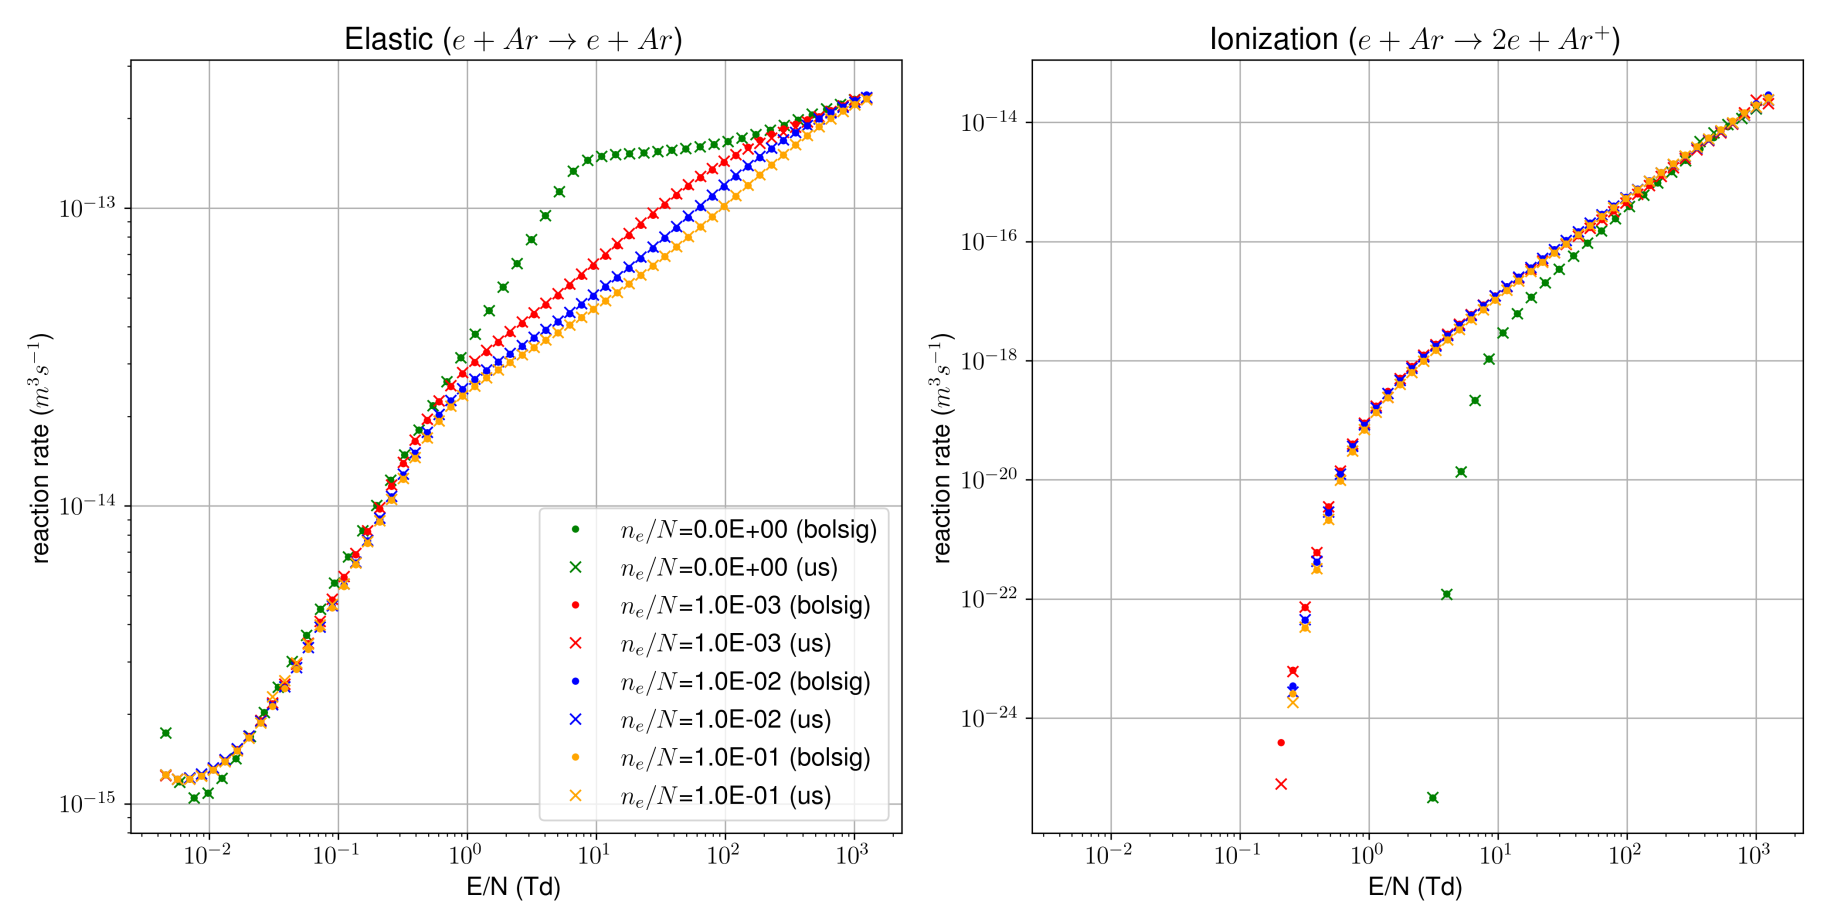
\includegraphics[width=0.9\textwidth]{pde_vs_bolsig_with_coulomb_collision1.png}}
%		%\only<+>{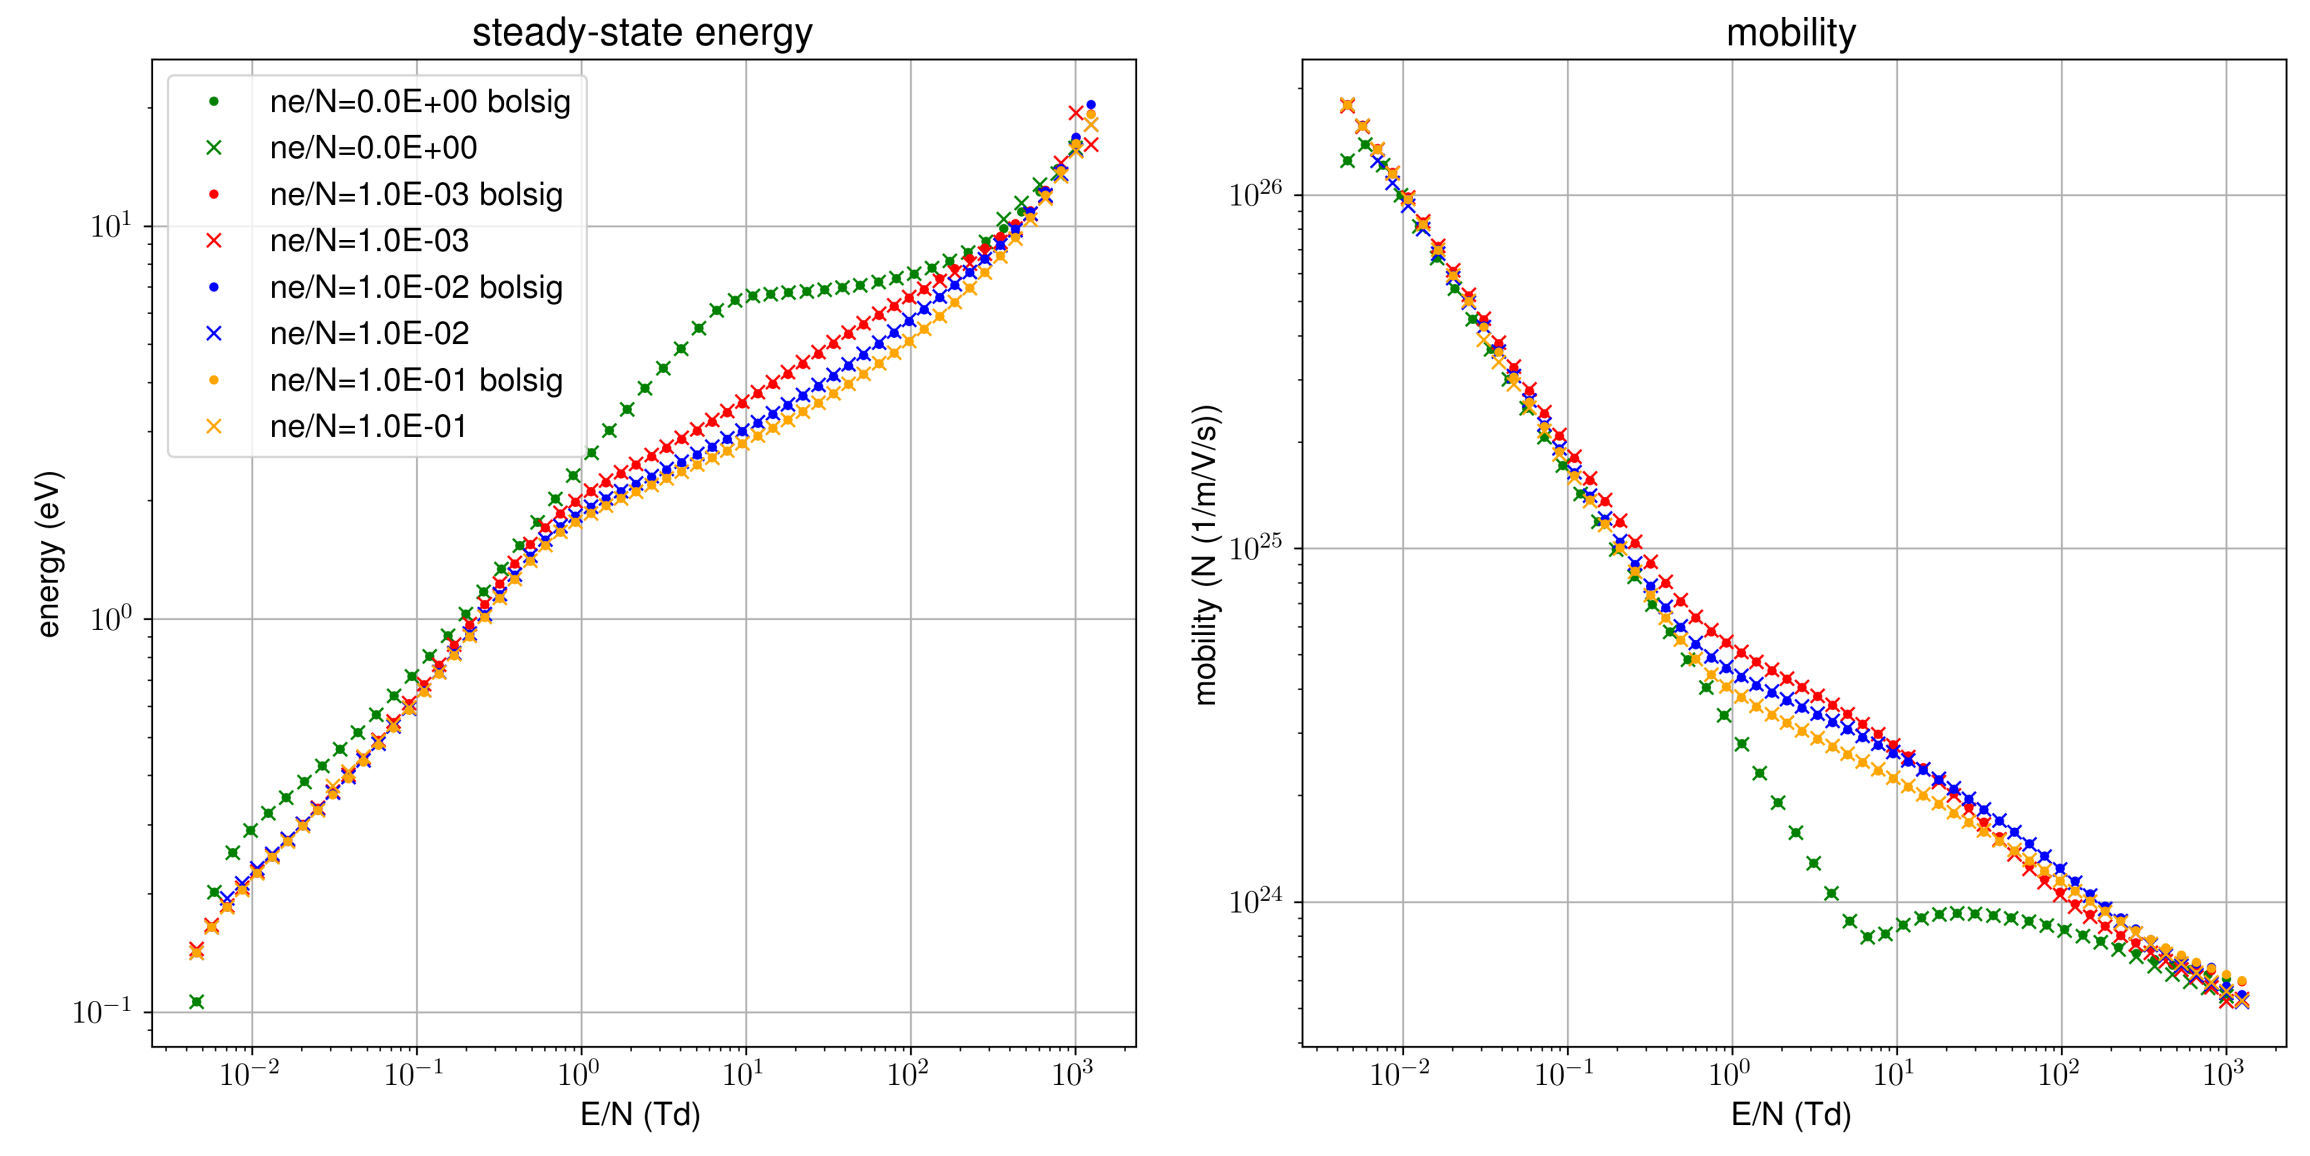
\includegraphics[width=0.9\textwidth]{pde_vs_bolsig_with_coulomb_collision2.png}}
%	\end{center}
%\end{frame}

\begin{frame}[fragile]
	\frametitle{Verification with Bolsig+}
	\vspace{-0.1in}
	\begin{center}
		\resizebox{0.68\textwidth}{!}{
			\renewcommand{\arraystretch}{1.2}
			\begin{tabular}{|p{1cm}|p{1cm}|c|c|c|c|c|c|}
			  \hline
			  \multirow{2}{1cm}{\textbf{$E/n_0$ (Td)}} & \multirow{2}{1cm}{\boldmath$n_e/n_0$} & \multicolumn{3}{c|}{\textbf{rel. error (deterministic vs. Bolsig+)}} & \multicolumn{3}{c|}{\textbf{rel. error (DSMC vs. Bolsig+)}} \\
			  % \hline
			  % \textbf{Inactive Modes} & \textbf{Description}\\
			  \cline{3-8}
			  & & \textbf{elastic} & \textbf{ionization} & \textbf{mobility} & \textbf{elastic} & \textbf{ionization} & \textbf{mobility}\\
			  %\hhline{~--}
			  \hline
			  1        & 0.0 & 7.11E-05 &    --	    & 4.10E-05	& 7.79E-03	& --  & 4.80E-03 \\
			  5        & 0.0 & 4.12E-04 & 3.74E-04	& 2.92E-06	& 7.77E-03	& 1.95E-03	& 1.87E-03   \\
			  20       & 0.0 & 5.76E-04 & 3.49E-03	& 2.98E-04	& 8.33E-03	& 4.77E-03	& 3.92E-03  \\
			  100      & 0.0 & 1.35E-03 & 2.74E-03	& 4.85E-03	& 1.14E-02	& 8.31E-03	& 5.05E-03   \\
			  \hline
			  1        & $10^{-3}$ & 9.40E-03	& 4.40E-03	& 7.99E-03	& 6.23E-03	& 7.61E-03	& 3.17E-03  \\
			  5        & $10^{-3}$ & 1.52E-02	& 4.12E-03	& 1.83E-04	& 5.90E-03	& 6.59E-03	& 5.89E-04  \\
			  20       & $10^{-3}$ & 1.69E-02	& 1.46E-02	& 1.13E-02	& 8.17E-03	& 1.09E-02	& 4.73E-03   \\
			  100      & $10^{-3}$ & 9.11E-03	& 1.87E-02	& 1.65E-02	& 1.50E-02	& 2.42E-02	& 1.75E-02   \\
			  \hline
			  1        & $10^{-2}$ & 4.88E-03	& 1.20E-02	& 9.94E-03	& 8.66E-03  & 1.38E-02  & 4.98E-03   \\
			  5        & $10^{-2}$ & 7.85E-03	& 8.73E-03	& 9.56E-03	& 4.82E-03  & 4.66-03  & 4.23E-03    \\
			  20       & $10^{-2}$ & 1.13E-02	& 4.57E-03	& 6.19E-03	& 5.36E-03  & 5.72E-03  & 2.10E-03   \\
			  100      & $10^{-2}$ & 1.19E-02	& 9.93E-03	& 7.76E-03	& 1.04E-02  & 2.05E-02  & 1.38E-02  \\
			  \hline
			  1        & $10^{-1}$ & 1.72E-03	& 8.17E-03	& 5.31E-03	& 5.80E-03  & 3.22E-02  & 6.75E-03  \\
			  5        & $10^{-1}$ & 2.42E-03	& 7.80E-03	& 7.74E-03	& 3.41E-03  & 3.03E-04  & 8.80E-03   \\
			  20       & $10^{-1}$ & 3.84E-03	& 7.97E-03	& 8.41E-03	& 3.30E-03  & 1.08E-02  & 9.56E-03   \\
			  100      & $10^{-1}$ & 4.76E-03	& 9.80E-04	& 1.89E-03	& 5.49E-03  & 5.59E-03  & 2.64E-03   \\
			  \hline
			\end{tabular}}
		% \resizebox*{0.63\textwidth}{!}{
		% \renewcommand{\arraystretch}{1.2}
		% \begin{tabular}{|p{1cm}|p{1cm}|c|c|c|c|c|c|}
		% 	\hline
		% 	\multirow{2}{1cm}{\textbf{$E/n_0$ (Td)}} & \multirow{2}{1cm}{\boldmath$n_e/n_0$} & \multicolumn{6}{c|}{\textbf{relative error}}  \\
		% 	% \hline
		% 	% \textbf{Inactive Modes} & \textbf{Description}\\
		% 	\cline{3-8}
		% 	& & \textbf{energy} &\textbf{mobility} & \textbf{elastic} & \textbf{ionization} & {$\mathbf{f_0(\varepsilon)}$} & {$\mathbf{f_1(\varepsilon)}$}\\
		% 	\hline
		% 	1	  &  0 & 	3.40E-11 & 	3.30E-11	&  5.74E-11	&   -	     &   6.42E-08	&1.99E-07\\
		% 	5	  &  0 & 	2.01E-10 & 	8.67E-10	&  2.69E-10	& 1.05E-08 &   1.08E-06	&3.77E-06\\
		% 	20	&  0 &  3.64E-10 & 	1.55E-09	&  6.08E-10	& 1.58E-08 &   1.78E-07	&2.50E-06\\
		% 	100 &  0 & 	3.62E-09 & 	5.10E-09	&  7.73E-09	& 1.20E-07 &   6.51E-07	&3.32E-06\\
		% 	\hline                  
		% 	1   &	$10^{-3}$ &	6.69E-07 &	7.21E-07 &	9.77E-07 &	4.77E-05 &	5.82E-07 &	1.28E-06\\
		% 	5   &	$10^{-3}$ &	9.71E-08 &	1.08E-07 &	1.40E-07 &	1.59E-06 &	1.22E-07 &	2.00E-07\\
		% 	20  &	$10^{-3}$ &	2.02E-09 &	4.09E-09 &	4.35E-09 &	7.94E-08 &	5.89E-07 &	5.23E-07\\
		% 	100 &	$10^{-3}$ &	6.30E-09 &	4.08E-08 &	1.33E-09 &	2.21E-08 &	1.69E-05 &  1.82E-05\\
		% 	\hline
		% 	1   &	$10^{-2}$ &	9.57E-06 &	1.07E-05 &	1.39E-05 &	3.36E-04 &	8.29E-06 &	1.94E-05\\
		% 	5   &	$10^{-2}$ &	4.04E-07 &	4.32E-07 &	5.87E-07 &	9.27E-06 &	3.65E-07 &	7.97E-07\\
		% 	20  &	$10^{-2}$ &	6.97E-08 &	6.73E-08 &	8.67E-08 &	1.76E-06 &	1.70E-07 &	2.23E-07\\
		% 	100 &	$10^{-2}$ &	4.04E-08 &	5.47E-08 &	4.67E-08 &	1.76E-07 &	3.05E-06 &	1.67E-06\\
		% 	\hline
		% 	1   &	$10^{-1}$ &	8.13E-05 &	1.07E-04 &	1.17E-04 &	1.69E-03 &	7.04E-05 &	1.94E-04\\
		% 	5   &	$10^{-1}$ &	3.34E-06 &	4.23E-06 &	4.84E-06 &	5.24E-05 &	2.89E-06 &	7.61E-06\\
		% 	20  &	$10^{-1}$ &	7.67E-07 &	8.58E-07 &	1.04E-06 &	1.07E-05 &	6.82E-07 &	1.62E-06\\
		% 	100 &	$10^{-1}$ &	4.04E-08 &	1.79E-08 &	2.06E-08 &	6.06E-07 &	5.21E-07 &	7.14E-07\\
		% 	\hline
		%   \end{tabular}}
		%\caption{Deterministic approach self convergence and comparison with the Bolsig code}
	\end{center}
\end{frame}



\begin{frame}
	\frametitle{Beyond two-term approximation}
	\vspace{-0.25in}
	% \begin{center}
	% 	%\includegraphics[width=0.6\textwidth]{mt_verification.png}
	% \end{center}
	\begin{center}
		\includegraphics[width=0.32\columnwidth]{mf_verification_0.pdf}
		\includegraphics[width=0.32\columnwidth]{mf_verification_2.pdf}
		\includegraphics[width=0.32\columnwidth]{mf_verification_3.pdf}
	\end{center}
	\begin{itemize}
		\item $E/N$ = 500Td , $T_g$=0K
	\end{itemize}
\end{frame}

\begin{frame}
	\frametitle{Application to plasma modeling}
		\begin{columns}
		\begin{column}{0.48\textwidth}
			\textbf{Plasma application}
			\footnotesize
			\begin{align*}
				&\partial_t n_i + \nabla_{\vect{x}} \cdot \vect{J_{n_i}}  = k_i n_0 n_i  \color{gray}{\text{ in } \Omega_x \times (0,T]}\\
				%\partial_t n_0 + \nabla_{\vect{x}} \cdot \vect{J_{n_0}}  = -k_i n_0 n_i \text{ in } \Omega_x \times (0,T]\\
				&\text{conservation of mass, momentum} \\
				&\quad  \text{and energy for } \vect{u}, n_0, T_g \\
				%\text{conservation of momentum for }  r^{+}, Ar  \\
				&\text{Maxwell's equations for } \vect{E}
			\end{align*}
			\begin{itemize}
				%\item $T_g=T_e$ %Assumes local thermodynamic equilibrium, (i.e., $T_e = T_g$) and quasi-neutrality (i.e., $n_e=n_i$)
				%\item Quasi-neutrality: $n_e = n_i$ 
				\item electron kinetic coefficients ~ closure model (i.e., $k_i \approx$ Maxwellian EEDF at $T$)
			\end{itemize}
		\end{column}
		\begin{column}{0.48\textwidth}
			\textbf{Plasma + electron-Boltzmann}
			%\vspace{0.25in}
			\footnotesize
			\begin{align*}
				&\partial_t n_i + \nabla_{\vect{x}} \cdot \vect{J_{n_i}}  = k_i n_0 n_i  \color{gray}{\text{ in } \Omega_x \times (0,T]}\\
				%\partial_t n_0 + \nabla_{\vect{x}} \cdot \vect{J_{n_0}}  = -k_i n_0 n_i \text{ in } \Omega_x \times (0,T]\\
				&\text{conservation of mass, momentum} \\
				&\quad  \text{and energy for } \vect{u}, n_0, T_g \\
				%\text{conservation of momentum for }  r^{+}, Ar  \\
				&\text{Maxwell's equations for } \vect{E}\\
				&\partial_t f  + \vect{v} \cdot \nabla_{\vect{x}} f -\frac{\vect{E} q}{m} \cdot \nabla_{\vect{v }}f = C(f, n_0, n_i, T_g) \color{gray}{\text{ in } \Omega_x \times \Omega_v \times (0,T]}
			\end{align*}
			\begin{itemize}
				\item Currently we consider 0D-BTE problem
				%\item $T_e \sim \int_{\vect{v}} \norm{\vec{v}}^2 \hat{f} \diff{\vect{v}}$
				%\item Quasi-neutrality: $n_e = n_i$ 
				\item $k_i = \int_{\vect{v}} \sigma(\norm{\vect{v}}) \hat{f} \diff{\vect{v}}$ where $\hat{f} = \frac{f}{\int_{\vect{v}} f \diff{\vect{v}}}$
				%\item 7D problem
			\end{itemize}
		\end{column}
	\end{columns}
\begin{itemize}
	\item \textcolor{orange}{Current application: Inductively coupled plasma torch simulations} 
\end{itemize}
\end{frame}

\begin{frame}
	\frametitle{Batched 0D-BTE}
	%\vspace{-0.1in}
	\begin{itemize}
		\item 0D--BTE maps $(E/N, T_g, ne/N, {n^{*}}_1/N, ... , {n^{*}}_k/N ) \rightarrow  f(t,\vect{v})$
		\item \textcolor{orange}{Amortize BTE v-space grid setup}
		\begin{center}
			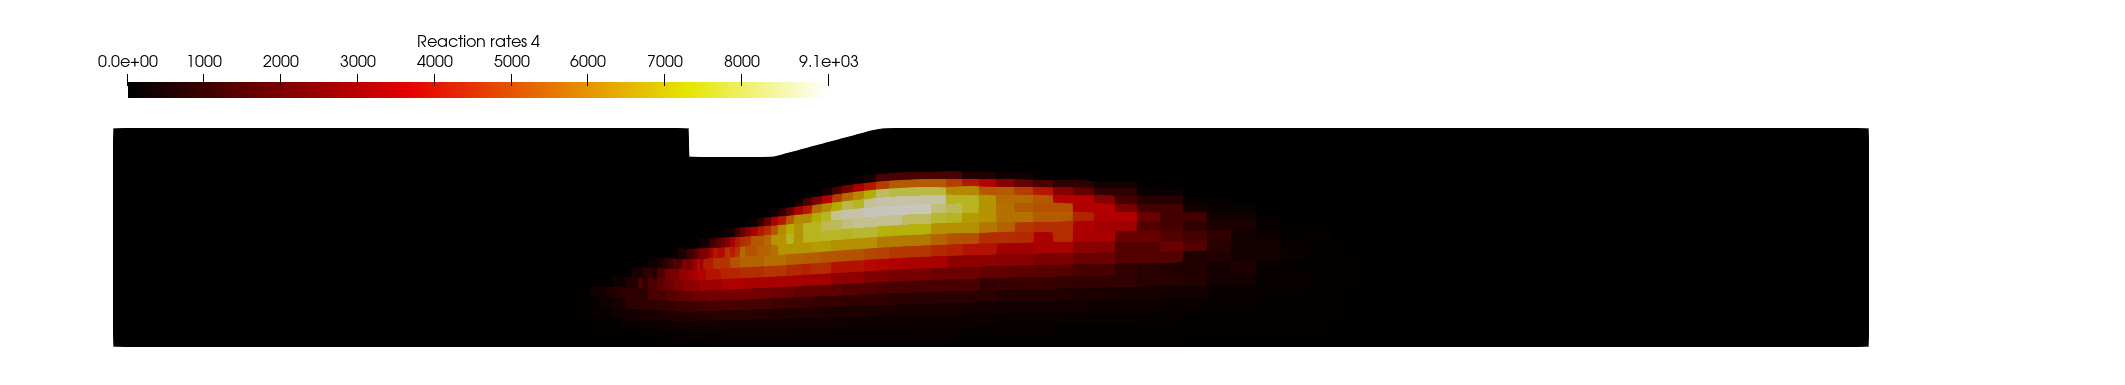
\includegraphics[width=0.95\textwidth]{tps_clustering.png}
		\end{center}
		\item BTE $\vect{v}$-discretization depends on $\vect{v}$-space truncation energy (use K-means based on $T_g$)
%		\item K-means clustering based on gas temperature $T_g(\vect{x})$. 
		\item With in each $T_g$ cluster again based on BTE input $(E/N, T_g, ne/N, {n^{*}}_1/N, ... , {n^{*}}_k/N )$ 
		\begin{itemize}
			\item 0D-interpolation for cluster members
		\end{itemize}
		%\item $\vect{v}$-space grid truncation $\quad\Rightarrow\quad$ $\overbar{T}_g$ $\quad\Rightarrow\quad$ set of $C_{en}, C_{ee}, A_v$ for cluster $i$%For each cluster EEDF is resolved up to $\varepsilon(\bar{T}_g)$
		% \begin{itemize}
			% 	\item Right-hand-side computation done by stacking BTE DoFs 
			% \end{itemize}
		{\footnotesize
			\begin{align*}
				\underbrace{C_{en}, C_{ee}, A_{v}}_{\text{pre-computed v-space operator for $T_g$-cluster}} \underbrace{\begin{bmatrix}
						%\vdots & \vdots & \hdots &\vdots\\
						f_1    & f_2    & \hdots & f_{N_A} \\
						\vdots & \vdots & \hdots &\vdots
				\end{bmatrix}}_{\text{batched DoFs for sub-cluster centers with in $T_g$-cluster}}
		\end{align*}}
	\end{itemize}
\end{frame}

\begin{frame}[fragile]
	\frametitle{Overview: 0D-Batched solver}
	\begin{columns}
		\begin{column}{0.48\textwidth}
			\begin{figure}
				\centering
				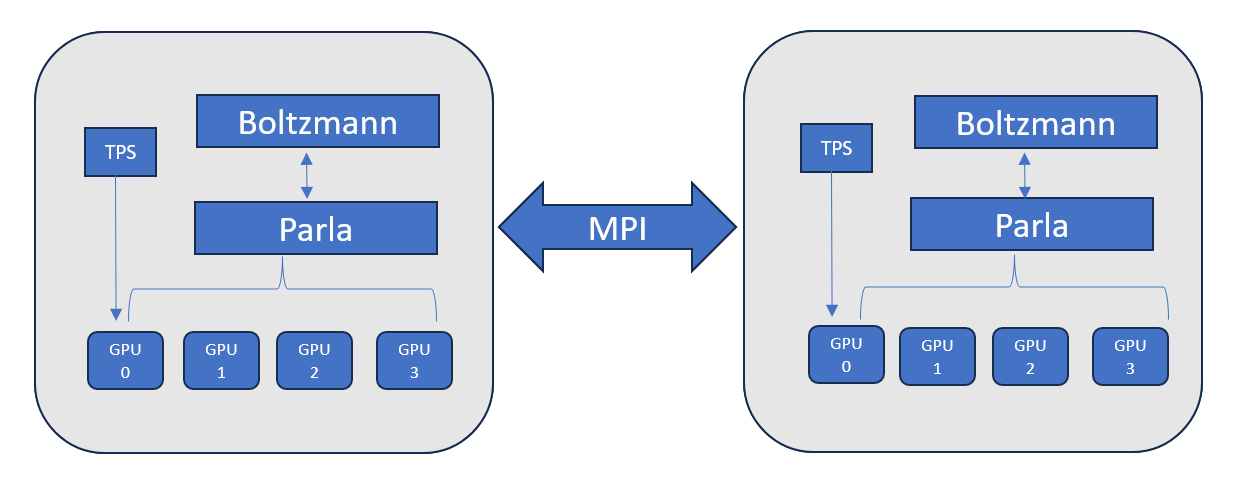
\includegraphics[width=1.0\columnwidth]{software_integration.png}
			\end{figure}		
		\end{column}
		\begin{column}{0.50\textwidth}
			\begin{mintedbox}{python}%[break at=.8\textheight]
ts_1 = TaskSpace("T")
for idx in range(num_clusters):
@spawn(ts_1[idx], placement=[p1[idx]], dependencies=ts_0[idx], vcus=0.0)
def t1():
  ff , qoi = bte.solve(idx, ...)
			\end{mintedbox}
		\end{column}
	\end{columns}
	\begin{itemize}
		%\item Information from Boltzmann to TPS is exchanged with interface class
		% \item Spatial points are clustered using heavy temperature
		% \item Different clusters $\rightarrow$ different $\epsilon_{max}$ truncation
		\item Computation between $\vect{v}$-space grids are embarrassingly parallel
		\item $\vect{v}$-space grid computations handed to \textbf{Parla} framework (Python based tasking system)
	\end{itemize}
\end{frame}


\begin{frame}[fragile]
	\frametitle{Parallel scalability: 0D-Batched BTE solver}
	%	TPS + 0D-Boltzmann problem setup
	\begin{itemize}
		\item Spatial points = 7598, DoF per point = 256, Total DoFs $\approx$ 2M, time for 200 implicit timesteps
		%\item runtime for 200 implicit timesteps
		\item Scalability study was performed in TACC's Lonestar 6 %$2\times 128$ AMD EPYC 7763 64-Core Processor with, 3-40GB Nvidia A100 GPU 
	\end{itemize}
	\begin{figure}
		\centering
		\begin{tikzpicture}
			\begin{axis}[
				width=10cm,
				height=5cm,
				ylabel={runtime (s)},
				xlabel={GPUs},
				symbolic x coords={3,6,12},
				xtick=data,
				grid=major
				]
				\addplot[-,mark=o,blue,thick] table[x={gpus}, y ={solve_max} ]{{../2023-11-08-PSAAP-Review/ls6/tpp_0d2v_ss.dat}};
				%\legend{Data1,Data2,Data3}
			\end{axis}
		\end{tikzpicture}
	\end{figure}
	\begin{itemize}
		\item 0D-Boltzmann grid setup $\approx$ 20s (independent of number of compute nodes)
		\item Parallel efficiency 78\%, 82\% $\rightarrow$ better load-balance with increasing partitions
	\end{itemize}
\end{frame}

\begin{frame}
	\frametitle{1D-space BTE}
	\begin{equation}
		\partial_t f + v\cos(\vtheta) \partial_z f -\frac{qe \vect{E}}{m_e} \cdot \nabla_{\vect{v}} f = C(f)
	\end{equation}
	\begin{itemize}
	\item Use method of discrete ordinates in $\vtheta$, $f_{\vtheta_j} = f(v, \vtheta_j, z, t)$
	\begin{align}
	\tiny
	&\partial_t f_{\vtheta_j} + v\cos\of{\vtheta_j} \partial_z f_{\vtheta_j} \nonumber \\
	&\quad = P (C + E) P^{T}\begin{bmatrix}
	f_{\vtheta_0}\\
	\vdots\\
	f_{\vtheta_{N_\vtheta}}\\
	\end{bmatrix} ; j=1,..., N_{\vtheta}	\label{eq:bte_discreate}
	\end{align}
	\item B-splines + Spherical in v-space +  Chebyshev-collocation %representation of $f$ in the velocity-space for collision and v-space advection
	%\item Chebyshev-collocation in space %Finite differences in $z$ direction
	\item Implicit time integration scheme
	\item First order operator splitting scheme for x-space and v-space
	\end{itemize}
\end{frame}

\begin{frame}
	\frametitle{1D-space BTE verification with PIC-DSMC}
	\begin{columns}
	\begin{column}{0.4\textwidth}
		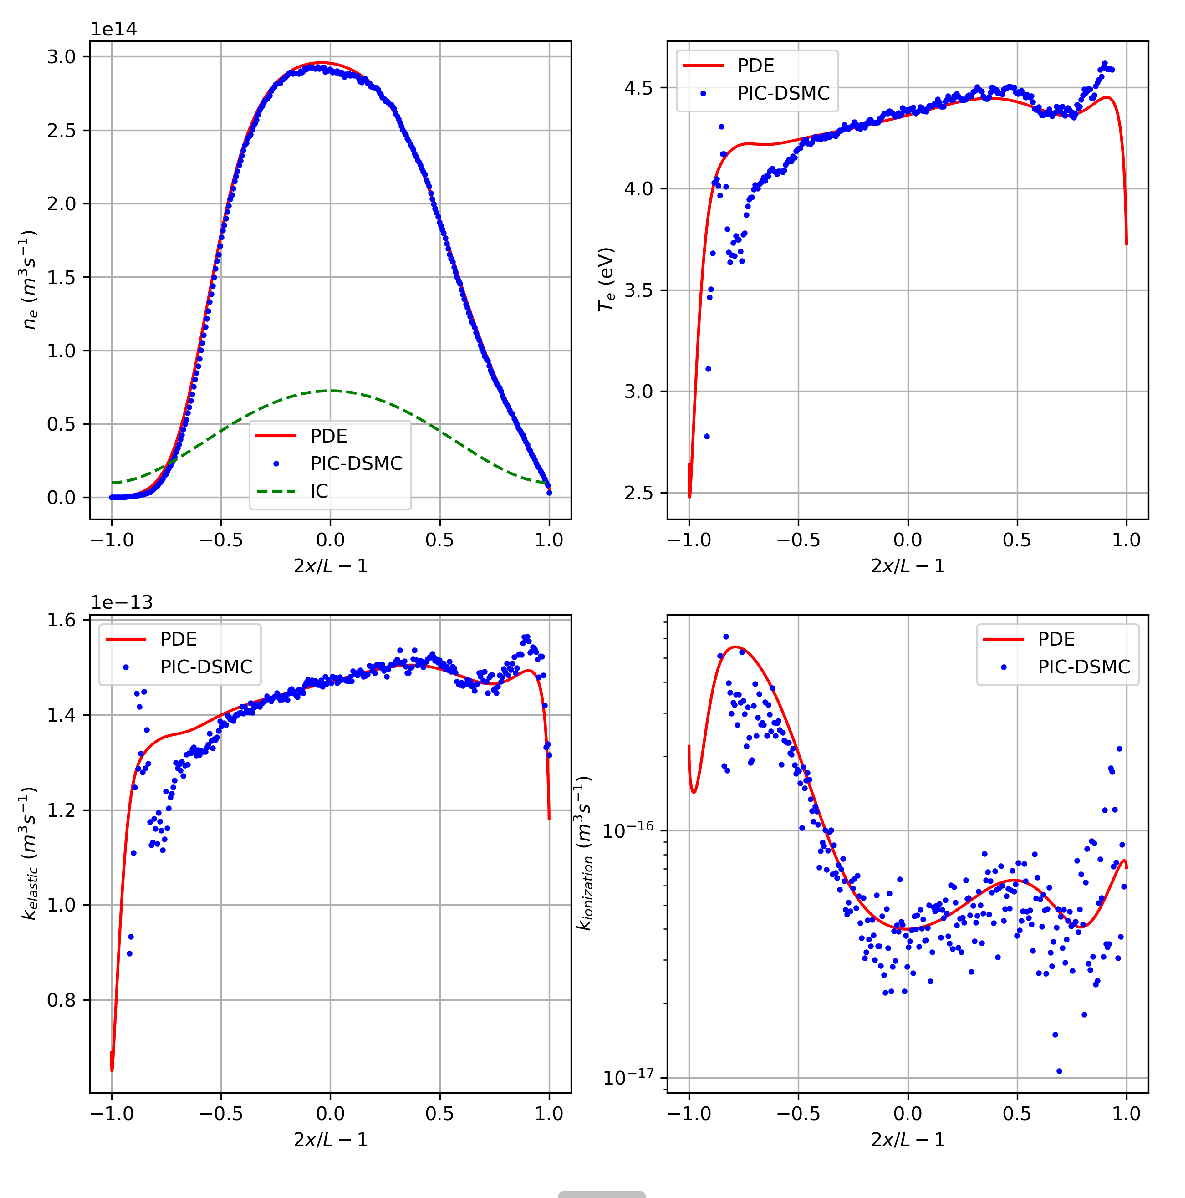
\includegraphics[width=1.1\textwidth]{1d_bte_pde_pic_dsmc.png}
	\end{column}
	\begin{column}{0.4\textwidth}
		\begin{itemize}
			\item $E(x, t) = E_0 \sin(2\pi f t)$, $f=13.56$ MHz and $E_0=10^4$ V/m
			\item Comparison between deterministic Vs. PIC-DSMC after 1 cycle
			\item Deterministic approach, $Nx=200, Nv=512 \times 6$ DoFs per grid point
			\item PIC-DSMC $Nx=300$ with 100K particles
		\end{itemize}
	\end{column}
\end{columns}
\end{frame}


\begin{frame}
	\frametitle{Summary \& future work}
	\begin{itemize}
		\item Summary
		\begin{itemize}
			\item v-space Galerkin with B-Splines + spherical harmonics with electron-heavy, electron-electron collisions
			\item Ability for multi-term expansion in $f$ (i.e., BC in space for 1D-space BTE)
			\item Batched 0D-space BTE solver for plasma applications
		\end{itemize}
		\item Future work
		\begin{itemize}
			\item Performance evaluation and optimization for batched solver
			\item 1D space Boltzmann equation
			\item Scaling to 2D, 3D BTE, reduce order modeling efforts
		\end{itemize}
	\end{itemize}
	\pause
	\begin{center}
		%Questions ? \\
		\Huge Thank You!
	\end{center}
\end{frame}


\end{document}
